\section{热传递的利用和防止}\label{sec:2-8}

热传递在日常生活和生产中有广泛的应用。
无论是利用热传递还是防止热传递,传导、对流、辐射这三种方式都应该考虑到,
因为在一般情况下,这三种方式是同时起作用的。

在需要利用热传递来散热的情况下,往往用热的良导体——金属来做热物体的外皮,以加强热的传导。
金属外皮的表面积尽可能做得大些,以增加辐射散热的面积。
此外,还要利用气体或者液体的对流来加快热传递。

汽车发动机工作的时候要发热,使机体的温度不断升高。
但是温度过高,发动机就不能正常工作,这就需要设法散热。
现在我们简单介绍汽车发动机的散热设备(图 \ref{fig:2-20})是怎样利用热传递的。

\begin{figure}[htbp]
    \centering
    \begin{minipage}{8cm}
    \centering
    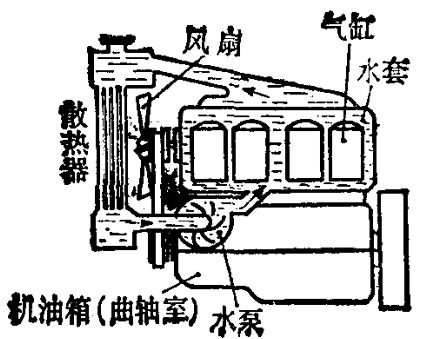
\includegraphics[width=7.5cm]{../pic/czwl2-ch2-20}
    \caption{汽车发动机的散热设备}\label{fig:2-20}
    \end{minipage}
    \qquad
    \begin{minipage}{6cm}
    \centering
    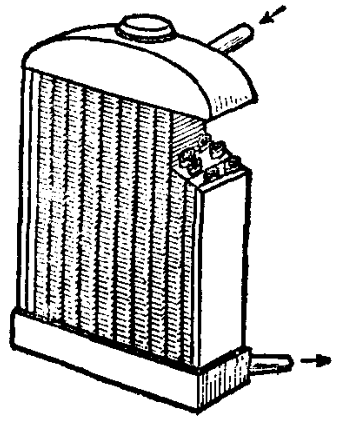
\includegraphics[width=5cm]{../pic/czwl2-ch2-21}
    \caption{散热器}\label{fig:2-21}
    \end{minipage}
\end{figure}


发动机气缸的外面装有水套,水套用上下两根管子跟散热器连通。
水套中的水受热膨胀,从上面的管子流入散热器。
散热器由许多金属管组成(图 \ref{fig:2-21}),金属管的外表面装有很多金属片。
从水套流来的热水经过传导把热传给金属片,金属片再把热向外辐射。
冷却后的水由下面的管子流回水套。
由于水的循环流动,热就不断地被带到散热器散出去。
可以看出,在这种装置里,热传递的三种方式都利用到了。

只利用水的对流来把热带到散热器,散热的速度还是比较慢的。
在功率较大的发动机里,还装有小型水泵,用来加快水的循环流动,使散热加快。
此外,在散热器的附近还装有风扇,把冷空气吹向散热器,这样也可以加快散热的速度。

在需要防止热传递的情况下,就要用相反的方法:
用热的不良导体来包扎物体,尽可能减小物体的表面积,并尽量避免对流的形成。

\begin{wrapfigure}[10]{r}{6cm}
    \centering
    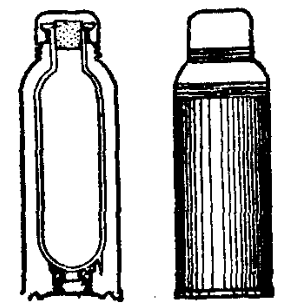
\includegraphics[width=5cm]{../pic/czwl2-ch2-22}
    \caption{保温瓶}\label{fig:2-22}
\end{wrapfigure}


保温瓶(图 \ref{fig:2-22})是防止热传递的例子。
它是一个有双层玻璃壁的瓶子,夹层里的空气已经抽得非常稀薄,接近真空。
夹层内的玻璃壁上镀了银,光亮的象镜子一样。
瓶口盖着软木塞。玻璃和软木都是热的不良导体。
夹层里没有空气,瓶口又盖着塞子,对流不可能发生。
镀银的光亮表面可以把从里面或外面辐射来的热反射回去。
这就是说,保温瓶把热传递的三种方式都尽可能避免了,所以它能够保温。



\lianxi

(1) 在冬天,用手摸户外的东西时,会觉得金属的比木头的凉。为什么?

(2) 盖棉被为什么觉得暖和?在夏天,用棉垫子把冰盖起来,冰是化得快些,还是化得慢些?为什么?

(3) 把滚开的水倒入一个厚玻璃容器时,玻璃容器常常会破裂。为什么?

(4) 图 \ref{fig:2-14} 和图 \ref{fig:2-15} 的实验为什么不发生对流?

(5) 拿一个装满了水的方框形玻璃管 $ABCD$(图 \ref{fig:2-23}),加热它的下角 $A$,玻璃管里的水将怎样流动?

\begin{figure}[htbp]
    \centering
    \begin{minipage}{7cm}
    \centering
    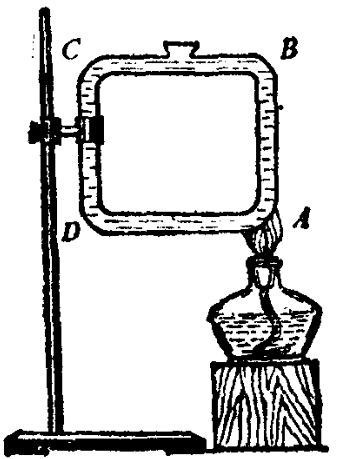
\includegraphics[width=5cm]{../pic/czwl2-ch2-23}
    \caption{}\label{fig:2-23}
    \end{minipage}
    \qquad
    \begin{minipage}{7cm}
    \centering
    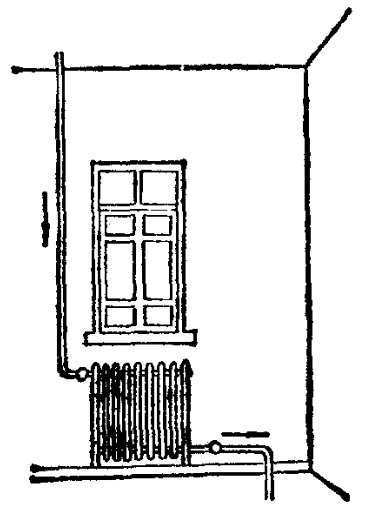
\includegraphics[width=5cm]{../pic/czwl2-ch2-24}
    \caption{}\label{fig:2-24}
    \end{minipage}
\end{figure}

(6) 在图 \ref{fig:2-24} 里,窗子下面是北方房间里冬季供暖用的暖汽片。有人想把它移到窗子上面,使房间宽敞些。
你认为他的想法有什么利弊,说明你的理由。

(7) 在阳光照射下,是脏雪化得快,还是干净雪化得快?

(8) 在夏季,把冰块放在保温瓶里比起放在普通的杯子里,化得快些,还是化得慢些?为什么?

(9) 了解你的教室在冬季(或夏季)采取了哪些取暖(或降温)的措施,并说明这些措施根据的是什么道理。

